\documentclass[10pt]{beamer}

\usetheme[progressbar=frametitle]{metropolis}
\usepackage{appendixnumberbeamer}

% ===================
% Metropolis BrownU Theme
% https://github.com/vskbellala/metropolis-brown
\usepackage{metropolisbrown}
% ===================

\usepackage{booktabs}
\usepackage[scale=2]{ccicons}

\usepackage{pgfplots}
\usepgfplotslibrary{dateplot}

\usepackage{xspace}
\newcommand{\themename}{\textbf{\textsc{metropolis}}\xspace}

\title{An Introduction to Minimum Principle}
%\subtitle{A modern beamer theme -- with a twist!}
% \date{\today}
\date{2024/07/24}
\author{Nuthasith (Nat) Gerdpratoom}
\institute{Control \& Optimization Laboratory}
\titlegraphic{\hfill\href{https://brown.edu}{
\includegraphics[height=2cm]{KU_en.png}}}

\begin{document}

\maketitle

\begin{frame}{Table of contents}
  \setbeamertemplate{section in toc}[sections numbered]
  \tableofcontents%[hideallsubsections]
\end{frame}

\section{Minimum Principle and Lagrange Multipliers}

\begin{frame}{Introduction}
  Optimal control involves minimizing a functional similar to ordinary optimization in finite dimensions. For unconstrained optimization, we find stationary points where the derivative of the function is zero. This concept extends to infinite dimensions in the calculus of variations.
\end{frame}

\begin{frame}{Lagrange Multipliers in Finite Dimensions}
  Consider an optimization problem with constraint \( g(x) = \mathbf{0} \), where \(g:\mathbb{R}^{m}\rightarrow \mathbb{R}^{d}\):
  \[
    \begin{aligned}
      &\underset{x}{\min}V(x) \\
      &\text{s.t. } g(x) = \mathbf{0}
    \end{aligned}
  \]
  In constrained optimization in \( \mathbb{R}^m \), we use Lagrange multipliers:
  \[
  \hat{V}(x, p) = V(x) + p^T g(x)
  \]
  where \( p \) is a Lagrange multiplier. If \( x^0, p^0 \) is a stationary point, then:
  \[
  \begin{aligned}
    \nabla_x \hat{V}(x^0, p^0) &= \nabla V(x^0) + \nabla g(x^0) p^0 = \mathbf{0}\\
    \nabla_p \hat{V}(x^0, p^0) &= g(x^0) = \mathbf{0}
  \end{aligned}
  \]
  \end{frame}

\begin{frame}{Lagrange Multipliers in Finite Dimensions}
  \begin{figure}
      \centering
      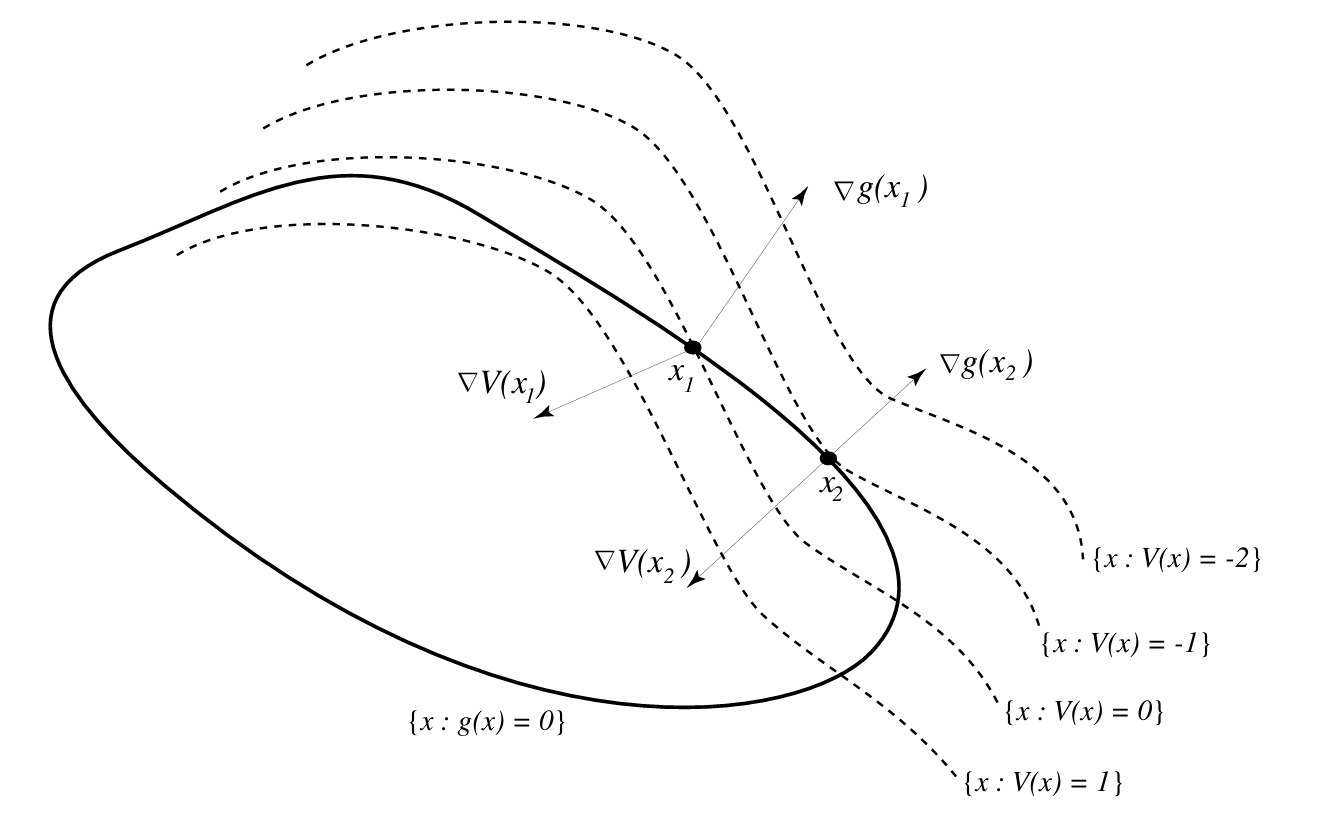
\includegraphics[width=0.8\textwidth]{photos/1.png}
      \caption{An optimization problem in \( \mathbb{R}^2 \) with a single constraint, $g(x)=0$.}
  \end{figure}
  \[
    \begin{aligned}
      \nabla_x \hat{V}(x^0, p^0) &= \nabla V(x^0) + \nabla g(x^0) p^0 = \mathbf{0}\\
      \nabla_p \hat{V}(x^0, p^0) &= g(x^0) = \mathbf{0}
    \end{aligned}
  \]
\end{frame}  

\begin{frame}{Generalizing to Infinite Dimensions}
  To generalize this to functional minimization, suppose that $F$ is a functional on $D^{r}[t_0,t_1]$, $F(z)$ is a real number, and $z \in D^{r}[t_0,t_1]$.
  We define the directional derivative:
  \[
    D_\eta F(z) = \lim_{\epsilon \to 0} \frac{F(z + \epsilon \eta) - F(z)}{\epsilon}
  \]
  A function \( z_0 \) is a stationary point of \( F \) if \( D_\eta F(z_0) = 0 \) for any \( \eta \).
  \begin{figure}
    \centering
    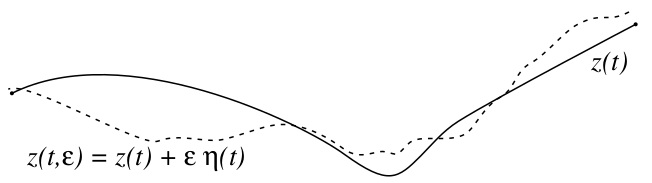
\includegraphics[width=0.7\textwidth]{photos/2.png}
    \caption{A Perturbation of function \(z\in D[t_{0},t_{1}]\)}
  \end{figure}
\end{frame}

\begin{frame}{Steps to Extend the Lagrange Multiplier Method}
\begin{enumerate}
    \item **Append state equations:** Define a new cost functional including the state dynamics:
    \[
    \hat{V}(x, u) = \int_{t_0}^{t_1} \ell \, dt + m(x(t_1)) + \int_{t_0}^{t_1} p^T (f - \dot{x}) \, dt
    \]
    \item **Integration by parts:** Eliminate the derivative of \( x \):
    \[
    \int_{t_0}^{t_1} p^T \dot{x} \, dt = \left[ p^T x \right]_{t_0}^{t_1} - \int_{t_0}^{t_1} \dot{p}^T x \, dt
    \]
    \item **Define the Hamiltonian:**
    \[
    H(x, p, u, t) = \ell(x, u, t) + p^T f(x, u, t)
    \]
\end{enumerate}
\end{frame}

\begin{frame}{Steps to Extend the Lagrange Multiplier Method (cont.)}
\begin{enumerate}
    \setcounter{enumi}{3}
    \item **Compute variations:** For perturbations \( x(t, \epsilon) = x^\circ(t) + \epsilon \eta(t) \) and \( u(t, \delta) = u^\circ(t) + \delta \psi(t) \), set \( \frac{d}{d\epsilon} \hat{V}(\epsilon) = 0 \) and \( \frac{d}{d\delta} \hat{V}(\delta) = 0 \).
    \item **Derive necessary conditions:** From the variations, derive the equations:
    \[
    \dot{p} = -\frac{\partial H}{\partial x}, \quad p(t_1) = \frac{\partial m}{\partial x}(x(t_1))
    \]
    \[
    \frac{\partial H}{\partial u} = 0
    \]
\end{enumerate}
\end{frame}

\begin{frame}{Deriving the Minimum Principle}
  Combine the steps to derive the Minimum Principle. If \( u^\circ \) is optimal, there exists a costate \( p(t) \) such that:
  \[
  u^\circ(t) = \arg \min_u H(x^\circ(t), p(t), u, t)
  \]
  The state and costate satisfy:
  \[
  \dot{x}^\circ = \frac{\partial H}{\partial p}, \quad \dot{p} = -\frac{\partial H}{\partial x}
  \]
  with boundary conditions:
  \[
  x(t_0) = x_0, \quad p(t_1) = \frac{\partial m}{\partial x}(x(t_1))
  \]
\end{frame}
  
\section{The Penalty Approach}
  
\begin{frame}[fragile]{The Penalty Approach}
  A third heuristic approach to the Minimum Principle involves relaxing the hard constraint \( \dot{x} - f = 0 \), and instead imposing a large, yet "soft" constraint.
  \[
  \hat{V}(x, u) = \int_{t_0}^{t_1} \ell(x(t), u(t), t) \, dt + \frac{k}{2} \int_{t_0}^{t_1} |\dot{x}(t) - f(x(t), u(t), t)|^2 \, dt + m(x(t_1))
  \]
  \end{frame}
  
  \begin{frame}[fragile]{Perturbation and Optimality}
  If \( (x_k, u_k) \) minimizes \( \hat{V}_k \), and letting \( (x^\circ, u^\circ) \) denote a solution to the original problem:
  \[
  \hat{V}_k(x_k, u_k) \leq \hat{V}_k(x^\circ, u^\circ) = V^\circ
  \]
  Assuming \( \ell \) and \( m \) are positive, this gives the uniform bound:
  \[
  \int_{t_0}^{t_1} |\dot{x}(t) - f(x(t), u(t), t)|^2 \, dt \leq \frac{2}{k} V^\circ
  \]
\end{frame}
  
\section{Application to LQR}
  
\begin{frame}[fragile]{Application to LQR}
  The LQR problem tests the Minimum Principle's utility for constructing optimal policies. Consider the general LTI model with quadratic cost:
  \[
  \dot{x} = Ax + Bu
  \]
  \[
  V = \int_{t_0}^{t_1} (x^T Q x + u^T R u) \, dt + x^T(t_1) M x(t_1)
  \]
\end{frame}
  
\begin{frame}[fragile]{Solving the LQR Problem}
  The Hamiltonian:
  \[
  H = x^T Q x + u^T R u + p^T (Ax + Bu)
  \]
  Control can be computed through:
  \[
  \nabla_u H = 0 \Rightarrow u = -\frac{1}{2} R^{-1} B^T p
  \]
  Resulting in:
  \[
  \dot{x} = Ax - \frac{1}{2} BR^{-1} B^T p
  \]
  \[
  \dot{p} = -\nabla_x H = -2Q x - A^T p
  \]
\end{frame}
  
\section{Nonlinear Examples}

\begin{frame}[fragile]{Nonlinear Examples}
  We solve some nonlinear problems where it is possible to obtain an explicit solution to the coupled state-costate equations given in the Minimum Principle. At the same time, we also give several extensions of this result.
\end{frame}
  
\begin{frame}[fragile]{Example 11.5.1: Bilinear System}
  Consider the control of a bilinear system, defined by the differential equation:
  \[
  \dot{x} = ux, \quad x(0) = x_0 > 0, \quad 0 \le u(t) \le 1
  \]
  Suppose the goal is to make \( x \) large while keeping the derivative of \( x \) small on average. The cost criterion is:
  \[
  V(u) = \int_0^{t_1} [u(\tau) - 1]x(\tau) \, d\tau
  \]
\end{frame}
  
\begin{frame}[fragile]{Optimal Control of Bilinear System}
  The Hamiltonian becomes:
  \[
  H(x, p, u, t) = x \{ u(p + 1) - 1 \}
  \]
  By the Minimum Principle, the optimal control is:
  \[
  u^\circ(t) = \begin{cases}
  1 & \text{if } p(t) + 1 < 0 \\
  0 & \text{if } p(t) + 1 > 0 \\
  \text{unknown} & \text{if } p(t) = -1
  \end{cases}
  \]
\end{frame}
  
\begin{frame}[fragile]{Costate and State Equations}
  The costate and state variables satisfy:
  \[
  \dot{p} = -(p + 1)u^\circ + 1
  \]
  \[
  \dot{x}^\circ = u^\circ x^\circ
  \]
  with the boundary conditions:
  \[
  x^\circ(0) = x_0, \quad p(t_1) = 0
  \]
\end{frame}
  
\begin{frame}[fragile]{Solving the Differential Equations}
  If \( t = t_1 \), then \( p(t) + 1 = 1 > 0 \) so \( u^\circ(t) = 0 \). By continuity, if \( t \approx t_1 \), then \( p(t) > 0 \), so \( u^\circ(t) = 0 \) and:
  \[
  \dot{p}(t) = 1 \quad \text{for } t \approx t_1 \implies p(t) = t - t_1
  \]
  For \( t < t_1 - 1 \), we have \( p(t) + 1 < 0 \) so \( u^\circ(t) = 1 \) and:
  \[
  \dot{p} = -p \quad \text{for } t < t_1 - 1 \implies p(t) = -e^{-t + t_1 - 1}
  \]
\end{frame}
  
\begin{frame}[fragile]{Bang-Bang Control}
  The optimal control is bang-bang:
  \[
  u(t) = \begin{cases}
  1 & \text{if } t < t_1 - 1 \\
  0 & \text{if } t > t_1 - 1
  \end{cases}
  \]
  The optimal state trajectory is:
  \[
  \dot{x}^\circ(t) = \begin{cases}
  x^\circ(t) & \text{if } t < t_1 - 1 \\
  0 & \text{if } t > t_1 - 1
  \end{cases}
  \]
  \[
  x^\circ(t) = \begin{cases}
  x_0 e^t & \text{if } t < t_1 - 1 \\
  x_0 e^{t_1 - 1} & \text{if } t > t_1 - 1
  \end{cases}
  \]
\end{frame}
  
\begin{frame}[fragile]{Minimum Principle with Constraints}
  Suppose \( x(t_1) \) is free, \( t_1 \) is fixed, and \( u^\circ \) is a solution to the optimal control problem (11.1) under the constraint \( u \in U \). The Minimum Principle with constraints states:
  \begin{enumerate}
      \item There exists a costate vector \( p(t) \) such that \( u^\circ(t) = \arg \min_{u \in U} H(x^\circ(t), p(t), u, t) \).
      \item The pair \( (p, x^\circ) \) satisfy the 2-point boundary value problem.
  \end{enumerate}
\end{frame}
  
\begin{frame}[fragile]{Example 11.5.1 with Constraints}
  Consider the bilinear system:
  \[
  \dot{x} = ux, \quad x(0) = x_0 > 0, \quad 0 \le u(t) \le 1
  \]
  with the cost criterion:
  \[
  V(u) = \int_0^{t_1} [u(\tau) - 1] x(\tau) \, d\tau
  \]
  The Hamiltonian:
  \[
  H(x, p, u, t) = x \{ u(p + 1) - 1 \}
  \]
  Optimal control:
  \[
  u^\circ(t) = \begin{cases}
  1 & \text{if } p(t) + 1 < 0 \\
  0 & \text{if } p(t) + 1 > 0
  \end{cases}
  \]
\end{frame}
  
\begin{frame}[fragile]{Costate and State Variables for Constrained Problem}
  The costate and state variables satisfy:
  \[
  \dot{p} = -(p + 1) u^\circ + 1
  \]
  \[
  \dot{x} = u^\circ x
  \]
  with boundary conditions \( x^\circ(0) = x_0 \), \( p(t_1) = 0 \).
\end{frame}
  
\begin{frame}[fragile]{Solving the Constrained Problem}
  If \( t \approx t_1 \):
  \[
  p(t) = t - t_1
  \]
  For \( t < t_1 - 1 \):
  \[
  p(t) = -e^{-t + t_1 - 1}
  \]
  The optimal control is bang-bang:
  \[
  u(t) = \begin{cases}
  1 & t < t_1 - 1 \\
  0 & t > t_1 - 1
  \end{cases}
  \]
\end{frame}
  
\begin{frame}[fragile]{Optimal State Trajectory for Constrained Problem}
  The optimal state trajectory:
  \[
  \dot{x}^\circ(t) = \begin{cases}
  x^\circ(t) & t < t_1 - 1 \\
  0 & t > t_1 - 1
  \end{cases}
  \]
  \[
  x^\circ(t) = \begin{cases}
  x_0 e^t & t < t_1 - 1 \\
  x_0 e^{t_1 - 1} & t > t_1 - 1
  \end{cases}
  \]
\end{frame}
  
\begin{frame}[fragile]{Minimum Principle with Final Value Constraints}
  Suppose \( t_0, t_1, x(t_0) = x_0 \), and \( x(t_1) = x_1 \) are prespecified. The Minimum Principle with final value constraints states:
  \begin{enumerate}
      \item There exists a costate vector \( p(t) \) such that \( u^\circ(t) = \arg \min_u H(x^\circ(t), p(t), u, t) \).
      \item The pair \( (p, x^\circ) \) satisfy the 2-point boundary value problem.
  \end{enumerate}
\end{frame}
  
\begin{frame}[fragile]{Example 11.5.2: LQR Problem with Terminal State}
  Consider the LQR problem with the terminal state specified. The cost criterion is:
  \[
  V = \frac{1}{2} \int_0^{t_1} (x^T Q x + u^T R u) \, dt, \quad R > 0, Q \ge 0
  \]
  The Hamiltonian:
  \[
  H = p (A x + B u) + \frac{1}{2} (x^T Q x + u^T R u)
  \]
  The optimal control:
  \[
  u^\circ(t) = -R^{-1} B^T p(t)
  \]
\end{frame}
  
\begin{frame}[fragile]{Costate Equation for LQR Problem}
  The costate vector satisfies the differential equation:
  \[
  \dot{p}(t) = -\frac{\partial H}{\partial x} = -p^T A - x^T Q
  \]
  \[
  (x, p) = \begin{pmatrix}
  A & -BR^{-1}B^T \\
  -Q & -A^T
  \end{pmatrix} \begin{pmatrix}
  x \\
  p
  \end{pmatrix}
  \]
  with boundary conditions:
  \[
  x(t_0) = x_0, \quad x(t_1) = x_1
  \]
\end{frame}
  
\begin{frame}[fragile]{State Transition Matrix}
  Let \( \psi(t, \tau) \) denote the state transition matrix:
  \[
  \frac{d}{dt} \psi(t, \tau) = H(t) \psi(t, \tau), \quad \psi(t, t) = I
  \]
  Decompose \( \psi(t, \tau) \) as:
  \[
  \psi(t, \tau) = \begin{pmatrix}
  \psi_{11}(t, \tau) & \psi_{12}(t, \tau) \\
  \psi_{21}(t, \tau) & \psi_{22}(t, \tau)
  \end{pmatrix}
  \]
\end{frame}
  
\begin{frame}[fragile]{Solving for Optimal Control}
  Compute the initial condition \( p(t_0) = p_0 \) to find \( p(t) \) for all \( t \):
  \[
  x_1 = x(t_1) = \psi_{11}(t_1, t_0) x_0 + \psi_{12}(t_1, t_0) p_0
  \]
  Assuming \( \psi_{12}(t_1, t_0) \) is invertible, we have:
  \[
  p_0 = \psi_{12}(t_1, t_0)^{-1} (x_1 - \psi_{11}(t_1, t_0) x_0)
  \]
\end{frame}
  
\begin{frame}[fragile]{Optimal Control and State Trajectory}
  For all \( t \):
  \[
  p(t) = \psi_{21}(t, t_0) x_0 + \psi_{22}(t, t_0) p_0
  \]
  The optimal control is:
  \[
  u^\circ(t) = -R^{-1} B^T p(t)
  \]
  The optimal state trajectory is:
  \[
  x^\circ(t) = \psi_{11}(t, t_0) x_0 + \psi_{12}(t, t_0) p_0, \quad t \ge t_0
  \]
\end{frame}
  
\begin{frame}[fragile]{Minimum Principle with Free Terminal Time}
  Suppose \( t_0, x(t_0) = x_0 \) are fixed, and some components of \( x(t_1) \) are specified. The Minimum Principle with free terminal time states:
  \begin{enumerate}
      \item There exists a costate vector \( p(t) \) such that \( u^\circ(t) = \arg \min_u H(x^\circ(t), p(t), u, t) \).
      \item The pair \( (p, x^\circ) \) satisfy the 2-point boundary value problem with modified boundary conditions.
      \item The unspecified terminal time \( t_1 \) satisfies:
      \[
      \frac{\partial m}{\partial t}(x^\circ(t_1), t) + H(x^\circ(t_1), p(t_1), u^\circ(t_1), t_1) = 0
      \]
  \end{enumerate}
\end{frame}
  
\begin{frame}[fragile]{Example 11.5.3: Minimum Time Problem}
  Consider a single input linear state space model:
  \[
  \dot{x} = Ax + bu
  \]
  We wish to find \( u^\circ \) which drives \( x \) from \( x(0) = x_0 \) to \( x(t_1) = x_1 \) in minimum time, under the constraint \( |u(t)| \le 1 \). The cost criterion is:
  \[
  V(u) = t_1 = \int_0^{t_1} 1 \, dt
  \]
  The Hamiltonian is:
  \[
  H = 1 + p^T(Ax + bu)
  \]
\end{frame}
  
\begin{frame}[fragile]{Bang-Bang Control Law}
  Minimizing \( H \) gives a bang-bang control law:
  \[
  u^\circ(t) = \begin{cases}
  1 & \text{if } p(t)^T b < 0 \\
  -1 & \text{if } p(t)^T b > 0
  \end{cases}
  \]
  If \( A, b \) are time-invariant and the eigenvalues of \( A \) are real, distinct, and negative, then \( p(t)^T b \) changes sign at most \( n - 1 \) times, bounding the number of switching times for the optimal control.
\end{frame}
  
\begin{frame}[fragile]{Costate Equation for Minimum Time Problem}
  The costate equation is:
  \[
  \dot{p} = -\nabla_x H = -A^T p
  \]
  Using the final time boundary condition \( H|_{t=t_1} = 0 \):
  \[
  1 + p(t_1)^T A x^\circ(t_1) + p(t_1)^T b u^\circ(t_1) = 1 + p(t_1)^T A x^\circ(t_1) - |p(t_1)^T b| = 0
  \]
\end{frame}
  
\begin{frame}[fragile]{Example: Double Integrator}
  Consider the double integrator \( \ddot{y} = u \):
  \[
  A = \begin{pmatrix} 0 & 1 \\ 0 & 0 \end{pmatrix}, \quad b = \begin{pmatrix} 0 \\ 1 \end{pmatrix}
  \]
  The optimal control is:
  \[
  u^\circ(t) = -\text{sgn}(p(t)^T b) = -\text{sgn}(p_2(t))
  \]
\end{frame}
  
\begin{frame}[fragile]{Solving Costate Equations}
  From the costate equations, for constants \( c_1, c_2 \):
  \[
  p_1(t) = c_1, \quad p_2(t) = -c_1 t + c_2
  \]
  The optimal control is bang-bang:
  \[
  u^\circ(t) = \begin{cases}
  1 & \text{if } t < t_1 - 1 \\
  0 & \text{if } t > t_1 - 1
  \end{cases}
  \]
\end{frame}
  
\begin{frame}[fragile]{Optimal Trajectories}
  The optimal state trajectories follow quadratic paths:
  \[
  x_1(t) = \begin{cases}
  \frac{1}{2} (x_2(t))^2 + K_1 & \text{if } u^\circ(t) = 1 \\
  -\frac{1}{2} (x_2(t))^2 + K_2 & \text{if } u^\circ(t) = -1
  \end{cases}
  \]
\end{frame}
\end{document}
